\documentclass[12pt]{article}

\usepackage{amssymb,amsmath,mathtools, tikz, pifont, url}
\usepackage[hidelinks, hypertexnames=false]{hyperref}
\usepackage[utf8]{inputenc}
\usepackage[T1]{fontenc}
\usepackage[english]{babel}
\usepackage{setspace}
\usepackage{graphicx}
\usepackage{xcolor}
\usepackage{float}
\usepackage{csquotes}
%\usepackage{tikz}
\usepackage{geometry}
\usepackage{listingsutf8}

% RISC-V Assembler syntax and style for latex lstlisting package
% 
% These are risc-v commands as per our university (University Augsburg, Germany) guidelines.
%
% Author: Anton Lydike
%
% This code is in the public domain and free of licensing

% language definition
\lstdefinelanguage[RISC-V]{Assembler}
{
  alsoletter={.}, % allow dots in keywords
  alsodigit={0x}, % hex numbers are numbers too!
  morekeywords=[1]{ % instructions
    lb, lh, lw, lbu, lhu,
    sb, sh, sw,
    sll, slli, srl, srli, sra, srai,
    add, addi, sub, lui, auipc,
    xor, xori, or, ori, and, andi,
    slt, slti, sltu, sltiu,
    beq, bne, blt, bge, bltu, bgeu,
    j, jr, jal, jalr, ret,
    scall, break, nop
  },
  morekeywords=[2]{ % sections of our code and other directives
    .align, .ascii, .asciiz, .byte, .data, .double, .extern,
    .float, .globl, .half, .kdata, .ktext, .set, .space, .text, .word
  },
  morekeywords=[3]{ % registers
    zero, ra, sp, gp, tp, s0, fp,
    t0, t1, t2, t3, t4, t5, t6,
    s1, s2, s3, s4, s5, s6, s7, s8, s9, s10, s11,
    a0, a1, a2, a3, a4, a5, a6, a7,
    ft0, ft1, ft2, ft3, ft4, ft5, ft6, ft7,
    fs0, fs1, fs2, fs3, fs4, fs5, fs6, fs7, fs8, fs9, fs10, fs11,
    fa0, fa1, fa2, fa3, fa4, fa5, fa6, fa7
  },
  morecomment=[l]{;},   % mark ; as line comment start
  morecomment=[l]{\#},  % as well as # (even though it is unconventional)
  morestring=[b]",      % mark " as string start/end
  morestring=[b]'       % also mark ' as string start/end
}

% usage example:

% define some basic colors
\definecolor{mauve}{rgb}{0.58,0,0.82}

\lstset{
  % listings sonderzeichen (for german weirdness)
  literate={ö}{{\"o}}1
           {ä}{{\"a}}1
           {ü}{{\"u}}1,
  % basicstyle=\tiny\ttfamily,                    % very small code
  breaklines=true,                              % break long lines
  commentstyle=\itshape\color{green!50!black},  % comments are green
  keywordstyle=[1]\color{blue!80!black},        % instructions are blue
  keywordstyle=[2]\color{orange!80!black},      % sections/other directives are orange
  keywordstyle=[3]\color{red!50!black},         % registers are red
  stringstyle=\color{mauve},                    % strings are from the telekom
  identifierstyle=\color{teal},                 % user declared addresses are teal
  frame=l,                                      % black line on the left side of code
  language=[RISC-V]Assembler,                   % all code is RISC-V
  tabsize=4,                                    % indent tabs with 4 spaces
  showstringspaces=false                        % do not replace spaces with weird underlines
}

\geometry{
 left=2.5cm,
 right=2.5cm,
 top=2.5cm,
 bottom=3cm,
 footskip=1cm,
 bindingoffset=0mm
}

% \usepackage[nottoc]{tocbibind}
\usepackage[backend=bibtex, urldate=long, dateabbrev=false]{biblatex}

%\pagestyle{plain}

\let\origthelstnumber\thelstnumber
\makeatletter
\newcommand*\Suppressnumber{
  \lst@AddToHook{OnNewLine}{
    \let\thelstnumber\relax
   % \advance\c@lstnumber-\@ne\relax% Not really necessary
  }
}

\newcommand\Reactivatenumber[1]{
  \global\c@lstnumber#1
  \global\advance\c@lstnumber\m@ne\relax
  \lst@AddToHook{OnNewLine}{
  \let\thelstnumber\origthelstnumber
  }
}
\makeatother

% \setlength\parindent{0pt}

\makeatletter
\newcommand\HUGE{\@setfontsize\Huge{50}{60}}
\makeatother

\title{Bachelor's Thesis}

\setcounter{tocdepth}{3}

\newcommand{\quotes}[1]{``#1''}

% \bibliographystyle{plain}
\bibliography{references}

\begin{document}


% titlepage

\singlespacing
\thispagestyle{empty}
\begin{center}
\begin{minipage}{\linewidth}
\flushright
	      		 
\centering

%University logo
% 
\includegraphics[width=0.5\linewidth]{logo.png}\par
% \vspace{1.0cm}
% Title

\vspace*{\fill}
{\scshape{\Large Bachelor's Thesis\par}}

\vspace{1.5cm}
{\scshape{\LARGE \textbf{Exploring Reasoning\\
    Performance of RISC-V\\
    Software Models in BTOR2}\par}}

\large
\vspace{2.0cm}
by\\
\vspace{0.25cm}
    {\scshape{Nadir Fejzić}}\\
% \vspace{0.2cm}
% Student ID: 11910236\\


\vspace{1.5cm}
\noindent%\rule{\textwidth}{0.3pt}
submitted in partial fulfillment of the requirements\\
    for the degree of
    {\scshape{Bachelor of Science}}\\
    in {\scshape{Informatics}}

\vspace{1.5cm}

\noindent%\rule{\textwidth}{0.3pt}
\begin{center}
    Department of Computer Sciences\\
    Paris Lodron University of Salzburg\\
    Salzburg, Austria\\
\end{center}


\bigskip
\vspace{0.5cm}

Supervised by:\\
\vspace{0.25cm}
Univ.-Prof. Dipl.-Inform. Dr.-Ing. Christoph Kirsch
\end{minipage}

\vspace{1cm}

\today
\end{center}
\vspace*{\fill}

\newpage

%\onehalfspacing
% \fontsize{12}{12}\selectfont

\abstract{When working with software programs, we often want to ensure that
they uphold certain invariants. There are various techniques for this, such as
testing. However, testing is not exhaustive. Instead, we can reduce the problem
of proving that the program upholds invariants to the boolean satisfiability
problem. This reduction is done by encoding the program as a sequence of
boolean formulas - known as the model, and solving the satisfiability of the
resulting formula. Solving this problem is computationally expensive, as it is
NP-Complete. In this thesis, we explore how different parameters of the
generated models affect the performance of SAT solvers. In particular we
present a benchmarking toolbox, and run benchmarks for different memory
granularity parameters.}

% \vspace*{\fill}

%\doublespacing
\newpage
\tableofcontents
\newpage
%\onehalfspacing
%\fontsize{12}{12}\selectfont

%---------------------------------------------------------------------------------------------------------------------------------------
%---------------------------------------------------------------------------------------------------------------------------------------
%---------------------------------------------------------------------------------------------------------------------------------------

\section{Introduction}

One of the requirements for software programs is the correctness. Varying
techniques, such as testing, are used as an attempt to ensure the correctness
of written software. However, in order to prove that the program is correct,
one would have to test it with every possible input.

Doing that is not feasible for most of the practical programs. What we can do
instead, is to prove that program has the desired properties for any input.
Software programs are a series of machine instructions executed by a machine.
Instructions and memory access in a machine are implemented using logical gates
in hardware. These logical gates can be modelled as boolean formulas, which
means that programs can be modelled as boolean formulas as well.

We can take advantage of this fact, and reduce the problem of proving the
correctness of software programs to the boolean satisfiability problem. During
the conversion of program to a boolean formula (the model) we can add
constraints that model the desired properties of the program. Solving such
model gives us the answer whether the program satisfies all of the constraints,
and thus whether it possesses the desired properties. 

Generating such models can be computed linearly in the size of the program
(number of instrucitons). But since the model is a reduction of the correcntess
problem to a satisfiability problem, solving the model means solving the
satisfiability problem. The satisfiability problem is, however, NP-Complete.
This means that solving of such models is computationally expensive. 

When generating models, we can tweak different parameters in order to influence
its complexity. For example, machines contain circuits for memory access.
Depending on the size of each addressable memory block (memory granularity), we
need to access a different number of addresses. This means that, for smaller
memory blocks, more addresses are needed to access the whole memory, which
results in more complicated model of memory access. Larger memory granularity
is better in this regard, but worse in others. In general, extracting values
from memory that differ in number of bits from the used memory granularity
increases complexity. We might need to use bit-shifting and bit-masking to
extract the desired value. If our program has frequent access to values in
memory smaller than the configured memory granularity, then this adds more
complexity for each such memory access. So memory granularity might affect the
solving performance.

We can tweak parameters of models to analyze how these shifts in complexity
affect the performance of solvers. In this thesis we're particularly
interested in solving performance when using different combinations of memory
granularity for code and non-code memory segments. We also aim for a general
setup that can be used to test and benchmark models of the same program
generated using different parameters. 

\newpage

\section{Bounded model checking}

\subsection{Correctness of software programs}

Software programs are written with a particular goal in mind. We can create a 
specification that describes what the goal of the program is. If the program 
does what it's supposed to do as defined by the specification, we say that the
program is correct. Depending on the program and our requirements, we can define
different specifications for different types of correctness. For example, we can
check whether the program logically does what it's supposed to. This would be 
logical correctness. Another example is we can check whether the program
performs unsafe operations, such as accessing memory out of bounds. This would
be safety correctness and so on.

In the context of this thesis, correctness of the program is defined as:

\begin{itemize}
    \item Program does not terminate with a bad exit code
    \item Program terminates with a good exit code
    \item Program does not perform division by zero
    \item Program does not inhibit division overflow
    \item Program does not access any invalid memory address
    \item Program does not inhibit segmentation fault
\end{itemize}

However, testing for each of these properties for any input is problematic. If
our program has a single 8-bit integer as its input, we would have to test it 
with $2^{8}$ different inputs. For each bit added to the input, regardless
if as an additional input or as an additional bit to the existing input, we
double the number of tests. Testing with such large input space is not feasible
for most of programs.

Better approach is to prove that our program is correct for any given input. In
our case, each property we want to check for is a particular state we want our
program to reach. What we're interested in, is whether an input for the given
program exists, such that a machine reaches a certain state while it executes
that program. This is known as the state reachability problem. In this thesis
we further reduce the state reachability problem to the boolean satisfiability
problem. The formal definition of the problem we want to solve is called model.
The reduction is done in such a way, that our model is satisfiable if and only
if the state is reachable. This means that, if our model is satisfiable, our
program upholds the desired constraints.

\subsection{Reduction to SAT Problem}

A program is a series of instructions that can be executed by a particular
machine. The machine decodes instructions and executes them. Instructions can 
have various semantics such as arithmetic operations, memory access, branching,
and so on. By executing the instructions, machine changes its state. Minimal
amount of state that is changed for each instruction is the update of the
program counter. Apart from program counter, the machine can modify its
registers and main memory as well.

% We can define instructions as mappings from the current state to the next state.
% But is that relevant in this context?

\begin{figure}
    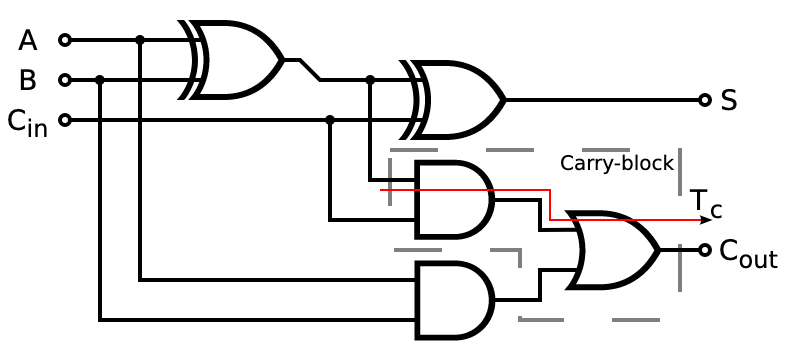
\includegraphics[width=\linewidth]{assets/full_adder_schematic.png}
    \centering
    \caption{
        Schematic of full adder implemented with two XOR gates, two AND gates,
        one OR gate.
    }
    \label{fig:full_adder_schematic}
\end{figure}

Instructions in machines are implemented using logical gates, such as AND, OR,
NOT and other gates. Logical gates are devices that perform boolean functions 
and are implementations of boolean formulas. In other words, we can model the
logical gates of the machine using boolean formulas. The logical circuit of one
instruction becomes a boolean formula in our model. An example of a 1-bit full
adder schematic can be seen in figure \ref{fig:full_adder_schematic}. The
schematic shows circuit logic for arithmetic addition with two 1-bit inputs $A$
and $B$, one 1-bit value from previous addition called carry in $C_{in}$ and it
computes the 1-bit sum $S$ and 1-bit carry out $C_{out}$ value in case of an
overflow. If we have a simple RISC-V program containing the following series of
instructions:
\begin{lstlisting}[language={[RISC-V]Assembler}, label=lst:example_riscv_program]
addi t0, zero, 4
addi t1, zero, 2
mul  t0, t0, t1
\end{lstlisting}
then we can model the program with the following operations:
\begin{lstlisting}[language=C, label=lst:example_model, caption=Example model]
t0_1 = 0    + 4    && pc_1 = pc_0 + 4 &&
t1_1 = 0    + 2    && pc_2 = pc_1 + 4 &&
t0_2 = t0_1 * t1_1 && pc_3 = pc_2 + 4 
\end{lstlisting}

So the small RISC-V program can be reduced to the series of operations in
listing \ref{lst:example_model}. What we encoded is a satisfiability modulo
theory formula (SMT-Formula). That is, we encoded the program as a series of
operations in theory of bit-vectors. This model is satisfiable if and only if
there exists an assigment of values to variables such that the formula is true.
For the SMT-Formula bit-vectors and arrays of bit-vectors are used. Bit-vectors
represent signed and unsigned integers of arbitrary bit-length, and bit vector
arrays are arrays of N-bit bit-vectors as values indexable by an M-bit
bit-vector. The model we encoded is an intermediate step, we need to further
reduce it to boolean formula.

If we recall the full adder schematic in figure \ref{fig:full_adder_schematic},
we can see that the logic gates correspond to the following boolean formulas:

\begin{align*}
    S	    &= A \oplus B \oplus C_{in} \\
    C_{out} &= (A \land B) \lor (C_{in} \land (A \oplus B))
\end{align*}

This is a series of boolean formulas that describe the behaviour of the 1-bit
full adder. For two bit full adder, we would have two sum outputs $S_1, S_2$,
one initial carry in $C_{in1}$, and the carry out of the first sum $C_{out1}$
would be the carry in to the second sum $C_{out1} = C_{in2}$. The same process
applies for full adder of values with arbitrary bit length. The series of
operations in listing \ref{lst:example_model} can be encoded in a similar
way. This technique of encoding semantics of arithmetic and bitwise operations
is called bit-blasing. We can add more constraints to the model that do not
come from the program, but rather specify whether the machine reaches a
particular state. For example, we can add constraints that check whether a
certain register of the machine (variable) contains the value $0$ and we
perform a division with that register. 

By doing so, we formulated a satisfiability problem, and by solving it we prove
that either our program does not perform division by zero for any given input,
or we get an example input for which the program performs division by zero. In
particular, by doing this, we reduced the state reachability problem to the
boolean satisfiability problem. Important observation is that the resulting 
boolean formula is finite and can model a finite number of executed
instructions, which makes our models bounded in the number of executed
instructions. This is the essence of bounded model checking.


\subsection{Complexity control with model parameters}

Model can be formulated for any given program with the technique of bit
blasting. There are multiple possibilities when generating model where certain
trade-offs can be made. In our models of the machine bit-vectors are used for
values and arrays of bit-vectors for main memory and registers. As already
mentioned, arrays contain bit-vectors of some fixed bit-length. If we want to
model M-bit memory with an array that contains N-bit bit-vectors we need an
address space of $2^{(M - N)}$ entries. More precisely, the array must be
indexed with a bit-vector of bit length $(M - N)$. Size of bit-vectors stored
in the array represent the memory granularity, the size of each memory block
our machine can access. By changing the memory granularity we can directly
impact the size of the array.

When accessing memory each memory block is addressable by an address, which is
a bit-vector in our case. Logical circuit exists for this purpose in machine as
well. Naively implemented, this could be a chain of something similar to
if-else statements. In reality machines use a logical circuit called
demultiplexer, which takes an input and routes it to one of several possible
outputs according to an input binary address \cite{horowitz1989art}.
Demultiplexer is another logical circuit that has $N$ inputs, each input having
two possible values, and $2^N$ outputs. By translating the circuit logic of
demultiplexer, we can model it as boolean formula as well, effectively
modelling memory access of the machine. Arrays used for memory representation
are indexed by N-bit bit-vectors, so the demultiplexer will have an $N$-bit
input value. Complexity of the resulting circuit logic directly depends on the 
size of the input, so choosing smaller memory granularity increases the
complexity of the model as well.

On the other hand, if we choose larger memory granularity, we can access the
whole memory with fewer addresses. Consequently, this reduces the memory access
circuits and therefore the complexity in corresponding part of our model.
However, it is not always the case that we need to access values in memory that
have the same size as our chosen granularity. When that's not the case, we have
to perform bit-shifting and bit-masking operations in order to load the correct
value. For example, if we want to load a 32-bit value from memory with 8-bit
granularity, we will have to access memory 4 times and perform bit-shifting to
store parts of value at the correct position. Smaller granularity in this case
results in four memory accesses through large circuit and four bit-shifting
operations. If we, however, want to load a 32-bit value from memory with 64-bit
granularity, we will have to perform a single load operation and bit-masking to
trim the value to the correct size. Larger granularity in this case reduces 
number of times we need to access the memory and reduces the number of
operations needed to correctly load the value.

In our models, we can control the memory granularity and therefore influence
the complexity of models in various parts. In particular, we can control two
different parts of memory: memory that holds the program instructions (code)
and memory that holds the data (data, heap and stack segments). In particular,
we try different combinations of code and data memory granularity.

\section{Model generation}

In order to properly model the machine, we need to generate a model that
resembles it. Models need to precisely define the semantic of memory access and
machine instructions. As we already mentioned, we do not generate boolean
formula directly, but rather an SMT-Formula first. We use a speical language
for this purpose called BTOR2.

\subsection{BTOR2 - brief introduction}

BTOR2 is an extension of BTOR, which is a format for quantifier-free formulas
over bit-vectors and arrays. BTOR2 extends BTOR by a set of additional features
and includes witness, invariant and fairness constraints and liveness
properties. BTOR2 supports defintion of sorts, which can be thought of as
types. For example, \texttt{sort bitvec 32} defines a sort of 32-bit
bit-vectors. Each line in BTOR2 format starts with an integer, which is either
a sort id for a sort definition, or node id for a node definition. Nodes in
BTOR2 can define operations such as addition, multiplication etc., or they can
be variable declaration, memory access, constraints and so on \cite{btor2}.

In listing \ref{lst:btor2_example} we can see an example of BTOR2 model. In 
first two lines we define two sorts, one is a 1-bit bit-vector with sort id 1,
and the other is a 32-bit bit-vector with sort id 2. In the following line we
have a node with node id 3 that defines an input variable \texttt{turn} of sort
with sort id 1, meaning that \texttt{turn} is a 1-bit bit-vector. In the next
line we define a constant 0 of sort with sort id 2. In next two lines we define
two 32-bit bit-vector state variables \texttt{a} and \texttt{b}, and then 
initialize them with previously defined constant 0. We then define a constant 1,
which we use to increment the state variables. We can observe that most of the
keywords first reference a sort id. The referenced sort id is the type of the
node, and the node itself evaluates to a certain value that we can reference by
the node's id. In nodes 12 and 13, we use an if-then-else construct, where we
evaluate to a certain value based on the condition. For state variable
\texttt{a} we check whether the value of node 3 is 1 (true), and if it is, the
node 12 evaluates to value of node 5, otherwise it evaluates to the value of
node 10. For state variable \texttt{b} we check whether the value of node 3 is
false (-3 negates the value of node 3), and if so we use the value of node 6,
otherwise value of node 11. Since nodes 5 and 6 are definitions of state
variables, using them means using whatever the current value of the variable
is. In nodes 14 and 15 we define the next function, which is the function that
updates the state variables, and these functions use the previously defined 
if-then-else nodes for the update. In next few lines we define a 32-bit
bit-vector constant 3, we have two nodes that check whether our state variables
have value 3. If both of them have value 3, the node 19 evaluates to 1 (true),
and in node 20 we define a bad state. The node 20 simply means, if the value of
node 19 is 1, then this bad state is reached. In listing \ref{lst:c_code} we 
can see the corresponding \texttt{C} code for the BTOR2 model.

\noindent\begin{minipage}{.45\textwidth}
\begin{lstlisting}[label=lst:btor2_example, caption={Example BTOR2 model},captionpos=b]
1 sort bitvec 1
2 sort bitvec 32
3 input 1 turn
4 zero 2
5 state 2 a
6 state 2 b
7 init 2 5 4
8 init 2 6 4
9 one 2
10 add 2 5 9
11 add 2 6 9
12 ite 2 3 5 10
13 ite 2 -3 6 11
14 next 2 5 12
15 next 2 6 13
16 constd 2 3
17 eq 1 5 16
18 eq 1 6 16
19 and 1 17 18
20 bad 19
\end{lstlisting}
\end{minipage}\hfill
\begin{minipage}{.5\textwidth}
\begin{lstlisting}[label=lst:c_code, language=c, caption={Corresponding code for the model},captionpos=b]
int main(void) {
    bool turn;

    unsigned int a = 0;
    unsigned int b = 0;

    while (1) {
        turn = read_bool();

        assert(!(a == 3 && b == 3));

        if (turn)
            a += 1;
        else
            b += 1;
    }
}
\end{lstlisting}
\end{minipage}

The BTOR2 format encodes the SMT-Formula. To solve the formula, we use a set of
tools that acompany the BTOR2 format contained in the project Boolector
\cite{DBLP:journals/jsat/NiemetzPB14}. In particular, we use the reference
implementation of a bounded model checker \texttt{btormc}. The bit-blasting of 
SMT-Formula is performed by the \texttt{btormc} before solving it. We run the
model checker by providing it the file containing BTOR2 model, and optionally
the upper bound. Upper bound option sets the maximal number of instructions
that can be checked. If the model checker terminates with no output, that means
that our program is does not satisfy the given constraints in the number of
instructions we chose as the upper bound. On the other hand, if the program
satisfies the constraints, a witness format is produced. We can see an example
output of witness format in listing \ref{lst:btor_witness}.

\begin{lstlisting}[label=btor_witness, caption={BTOR2 Witness Format for model in listing \ref{lst:btor2_example}}, captionpos=b]
sat
b0
@0
0 1 turn@0
@1
0 0 turn@1
@2
0 0 turn@2
@3
0 0 turn@3
@4
0 1 turn@4
@5
0 1 turn@5
@6
0 0 turn@6
.
\end{lstlisting}

The \texttt{sat} indicates that the model is satisfiable, \texttt{b0} is the 
satisfiable property with \texttt{b0} for 0-th bad property, that is the first
bad property that appears in the model. \texttt{@0} through \texttt{@6}
indicate the assignments of the inputs in frames 0 to 6, e.g., e.g., in frame
0 the 0-th input (first input defined in the BTOR2 model) \texttt{turn = 1} and
so on. Frame 6 is the last frame, where the bad property \texttt{b0} is
satisfied.

\subsection{\texttt{rotor} - tool of choice}

Generating BTOR2 models for programs is not done by hand. That would be tedious
and error prone, as models tend to be very large counting tens of thousands of
lines. Instead, we use tool capable of generating BTOR2 models. In particular,
we use \texttt{rotor}, which is a self-translating modeling
engine called based on \texttt{selfie} that translates full RISC-V code
including all of \texttt{selfie} and itself to BTOR2 and SMT-LIB formulae that
are satisfiable if and only if there is input to the code such that the code
exits with non-zero exit codes, performs division by zero, or accesses memory
outside of memory segments. Rotor also generates models that enable RISC-V code
synthesis \cite{gh:rotor}.

\subsubsection{Model Parameters and Checks}

\texttt{rotor} accepts multiple arguments and parameters that can be used to
adjust produced models. By default multiple checks are enabled in
\texttt{rotor}, and we have to explicitely disable them using following command
line argumnets:

\begin{itemize}
    \item \texttt{-Pnobadexitcode} - Disables check for bad exit code. Without
        this option, the model checker will report satisfiable if the program
        can terminate with the chosen bad exit code.
    \item \texttt{-Pgoodexitcode} - Enables check for good exit code. With this
        enabled, the model is satisfiable if the program can exit with some 
        exit code other than the chosen good exit code.
    \item \texttt{-Pnoexitcodes} - Disables checking whether multiple cores
        exit with the same exit code. If not present, model is satisfiable if
        different cores can exit with different exit codes.
    \item \texttt{-Pnodivisionbyzero} - Disables division by zero check, which
        checks whether an input for the program exists such that the program
        performs division by zero.
    \item \texttt{-Pnodivisionoverflow} - Disables check for division (or
        remainder) overflow. Without this option, model is satisfiable if an
        input exists such that program performs division with an overflow.
    \item \texttt{-Pnosegfaults} - Disables check for segfaults, which checks
        whether the program accesses memory outside of memory segments.
\end{itemize}

Apart from these checks, we can also modify some parameters of the model.
Models generated for benchmarking in this thesis are generated with following
parameters: 

\begin{itemize}
    \item \texttt{-bytestoread 1} - Input of the program is 1 byte
    \item \texttt{-cores 1} - Machine has a single core
    \item \texttt{-virtualaddressspace 32} - 32-bit virtual address space
    \item \texttt{-codewordsize X} - Granularity of the code memory segment,
        where \texttt{X} is the size of the code memory segment in bits
    \item \texttt{-memorywordsize X} - Granularity of the non-code memory
        segments (data, stack and heap), where \texttt{X} is the size of the
        memory segment in bits.
    \item \texttt{-heapallowance 4096} - Maximum heap size in bytes
    \item \texttt{-stackallowance 4096} - Maximum stack size in bytes
\end{itemize}

As we can see, the memory granularity of code and non-code memory segments can
be independently configured. This was used to generate models with different
combinations of code and non-code memory granularity. We can generate many 
models rather quickly, because the generation of models is linear to the size
of the input program. \texttt{rotor} accepts either \texttt{C*} source code,
binary compiled by \texttt{starc} or binary compiled by \texttt{gcc} as inputs.
In case of using binaries as input, they must be compiled for the
\texttt{RISC-V} architecture.


\section{Experiment setup}

\subsection{peRISCope - short outline of available functionality}

\texttt{peRISCope} is a benchmarking toolbox designed to make the process of 
parameterized model generation and benchmarking of model solving easier. The 
tool also supports parsing of BTOR2 witness format in order to provide more 
information, such as which property was satisfied, and transitions of inputs
through frames that satisfy said property. \texttt{peRISCope} accepts a
configuration file, which can be used to specify the parameters for models,
timeout for maximum duration of model solving, list of files for filtering, and
flags for \texttt{btormc}. The \texttt{peRISCope} performs multiple run. In
each run it reads the configuration, runs \texttt{rotor} with parameters of
that run which results in multiple models being generated in (specific)
\texttt{selfie} directory. Model generation is fast, so we can generate models
for all example files with no filtering. After the models are generated,
\texttt{btormc} is run on each model multiple times using \texttt{hyperfine}
\cite{Peter_hyperfine_2023}, measuring the time it took each time. Example of
the config file can be seen in listing 
\ref{lst:periscope_config}.

\begin{lstlisting}[label=lst:periscope_config, caption={Example peRISCope configuration file}, captionpos=b]
timeout: 300
files: # perform model checking only on files with these names
  - "division-by-zero-3-35-rotorized.btor2"
  - "invalid-memory-access-fail-2-35-rotorized.btor2"

runs: # model configuration flags for 'rotor'
  8-bit-codeword-size: "0 -codewordsize 8"
  16-bit-codeword-size: "0 -codewordsize 16"
  32-bit-codeword-size: "0 -codewordsize 32"
  64-bit-codeword-size: "0 -codewordsize 64"

\end{lstlisting}

\subsection{Workflow (peRISCope configuration, model generation, benchmarking, parsing of witness format, result files)}


\section{Experiment results}

\subsection{Results with binaries compiled with selfie}

\subsection{Results with binaries compiled with gcc}


\section{Conclusion and further work}

\bigskip

%---------------------------------------------------------------------------------------------------------------------------------------
%---------------------------------------------------------------------------------------------------------------------------------------
%---------------------------------------------------------------------------------------------------------------------------------------

\newpage

\printbibliography

\newpage

%\topskip0pt
\vspace*{\fill}
\begin{center}
    \textbf{\Huge Statement of Authentication}\\
\end{center}

\vspace{1cm}

I hereby declare that I have written the present thesis independently, without
assistance from external parties and without use of other resources than those
indicated. The ideas taken directly or indirectly from external sources
(including electronic sources) are duly acknowledged in the text. The material,
either in full or in part, has not been previously submitted for grading at
this or any other academic institution.\\

\vspace{1cm}

Salzburg,\today \hspace{0.5cm}\hrulefill\\
\vspace{-0.5cm}
\flushright Nadir Fejzić

\vspace*{\fill}
\end{document}
